
\newcommand{\tn}[1]{\mbox{\bf{#1}}}
\newcommand{\sig}{\mbox{\boldmath $\sigma \!\!$ \unboldmath}}
\newcommand{\bnabla} {\mbox{\boldmath $\nabla \!\!$ \unboldmath}}
\newcommand{\taubold} {\mbox{\boldmath $\tau \!\!$ \unboldmath}}
\newcommand{\f}{\ensuremath{f^{\theta}_r} }

\newcommand{\Texp}{\rm{exp}}
\newcommand{\Text}{\rm{ext}}
\newcommand{\Tint}{\rm{int}}
\newcommand{\Teq}{\rm{eq}}
\newcommand{\Delt}{\ensuremath{\Delta t}}
\newcommand{\Ep}{\ensuremath{\epsilon_p}}
\newcommand{\Epdot}[1]{\ensuremath{\dot{\epsilon}_{p#1}}}
\def\bfE{{\bf E}}
\newcommand{\BD}{\ensuremath{\boldsymbol{D}}}
\newcommand{\Half}{\ensuremath{\frac{1}{2}}}
\newcommand{\Bsig}{\ensuremath{\boldsymbol{\sigma}}}
\newcommand{\Bn}{\ensuremath{\boldsymbol{n}}}
\newcommand{\Bg}{\ensuremath{\boldsymbol{g}}}

\def\rmd{{\rm d}}
\def\rme{{\rm e}}
\def\rmf{{\rm f}}
\def\rmr{{\rm r}}
\def\rmR{{\rm R}}
\def\rms{{\rm s}}
\def\bfE{{\bf E}}
\def\bfF{{\bf F}}
\def\bff{{\bf f}}
\def\bfg{{\bf g}}
\def\bfI{{\bf I}}
\def\bfj{{\bf j}}
\def\bfm{{\bf m}}
\def\bfr{{\bf r}}
\def\bfx{{\bf x}}
\def\bfu{{\bf u}}
\def\rmg{{\rm g}}
\def\bfa{{\bf a}}
\def\bfG{{\bf G}}
\def\bfv{{\bf v}}
\def\tdot{{\textstyle\cdot}}

\section{MPM} \label{Sec:MPM}

\subsection{Introduction}

The material point method (MPM) was described by Sulsky et al.~\cite{sulskycmame,sulskycpc} as
an extension to the FLIP (Fluid-Implicit Particle) method of
Brackbill~\cite{brackbill-ruppel86}, which itself is an
extension of the particle-in-cell (PIC) method of
Harlow~\cite{harlow1963}.  Interestingly, the name ``material point method"
first appeared in the literature two years later in a description of
an axisymmetric form of the method~\cite{sulsky_axisym_1996}.  In both
FLIP and MPM, the basic idea is the same: objects are discretized into
particles, or material points, each of which contains all state data for the
small region of material that it represents.  This includes the position, mass, volume,
velocity, stress and state of deformation of that material.  MPM differs from
other so called ``mesh-free" particle methods in that, while each object
is primarily represented by a collection of particles, a computational mesh
is also an important part of the calculation.  Particles do not interact
with each other directly, rather the particle information is accumulated
to the grid, where the equations of motion are integrated forward in time.
This time advanced solution is then used to update the particle state.

The method usually uses a regular structured grid as a computational mesh.
While this grid, in principle, deforms as the material that it is representing
deforms, at the end of each timestep, it is reset to its original undeformed
position, in effect providing a new computational grid for each timestep.
The use of a regular structured grid for each time step has a number of
computational advantages.  Computation of spatial gradients is simplified.
Mesh entanglement, which can plague fully Lagrangian techniques, such as
the Finite Element Method (FEM), is avoided.  MPM has also been successful
in solving problems involving contact between colliding objects, having an
advantage over FEM in that the use of the regular grid eliminates the
need for doing costly searches for contact surfaces\cite{bard}.

In addition to the advantages that MPM brings, as with any numerical technique, it has its own set of shortcomings.  It is computationally more
expensive than a comparable FEM code.  Accuracy for MPM is typically lower
than FEM, and errors associated with particles moving around the computational
grid can introduce non-physical oscillations into the solution.  Finally,
numerical difficulties can still arise in simulations involving large
deformation that will prematurely terminate the simulation.  The severity of
all of these issues (except for the expense) has been significantly reduced
with the introduction of the Generalized Interpolation Material Point Method,
or GIMP\cite{bardgimp}.  The basic concepts associated with GIMP will be
described below.  Throughout this document, MPM (which
ends up being a special case of GIMP) will frequently be referred to
interchangably with GIMP.

In addition, MPM can be incorporated with a multi-material CFD algorithm
as the structural component in a fluid-structure interaction formulation.
This capability was first demonstrated in the CFDLIB codes from
Los Alamos by Bryan Kashiwa and co-workers\cite{kashiwa2000}.  There, as
in the Uintah-MPMICE component,
MPM serves as the Lagrangian description of the solid
material in a multimaterial CFD code.  Certain elements of the
solution procedure are based in the Eulerian CFD algorithm, including
intermaterial heat and momentum transfer as well as satisfaction
of a multimaterial equation of state.  The use of a Lagrangian method
such as MPM to advance the solution of the solid material eliminates
the diffusion typically associated with Eulerian methods.  The Uintah-MPM
component will be described in later chapter of this manual.

Subsequent sections of this chapter will first give a relatively brief
description of the MPM and GIMP algorithms.  This will, of course, be
focused mainly on describing the capabilities of the Uintah-MPM component.
This is followed by a section that attempts to relate the information in
Section~\ref{Sec:AlgDesc} to the implementation in Uintah.
Following that is a description of the information that goes into an input
file.  Finally, a number of examples are provided, along with representative
results.

\subsection{Algorithm Description} \label{Sec:AlgDesc}

Time and space prohibit an exhaustive description of the theoretical
underpinnings of the Material Point Method.   Here we will concentrate
on the discrete equations that result from applying a weak form analysis
to the governing equations.  The interested reader should
consult \cite{sulskycmame,sulskycpc} for the development of these discrete
equations in MPM, and \cite{bardgimp} for the development of the equations
for the GIMP method.  These end up being very similar, the differences in
how the two developments affect implementation will be described in
Section~\ref{gimp_mpm}.

In solving a structural mechanics problem with MPM, one begins by discretizing
the object of interest into a suitable number of particles, or ``material
points".  ({\bf Aside:}  What constitutes a suitable number is something of an open
question, but it is typically advisable to use at least two particles in each
computational cell in each direction, i.e. 4 particles per cell (PPC) in 2-D,
8 PPC in 3-D. In choosing the resolution of the computational grid, similar
considerations apply as for any computational method (trade-off between
time to solution and accuracy, use of resolution studies to ensure convergence
in results, etc.).)  Each of these particles will carry, minimally, the
following variables:
\begin{enumerate}

\item position - $\bfx_p$
\item mass - $m_p$
\item volume - $v_p$
\item velocity - $\bfv_p$
\item stress - $\sig_p$ 
\item deformation gradient - $\bfF_p$

\end{enumerate}

The description that follows is a recipe for advancing each of these
variables from the current (discrete) time $n$ to the subsequent
time $n+1$.  Note that particle mass, $m_p$, typically remains constant
throughout a simulation unless solid phase reaction models are utilized,
a feature that is not present in Uintah-MPM.  (Such models are available
in MPMICE, see Section \ref{Sec:MPMICE}.)  It is also important to point
out that the algorithm for advancing the timestep is based on the so-called
Update Stress Last (USL) algorithm.  The superiority of this approach over
the Update Stress First (USF) approach was clearly demonstrated by Wallstedt
and Guilkey \cite{WallstedtJCP}.  USF was the formulation used in Uintah
until mid-2008.

The discrete momentum equation that results from the weak form is given as:
\begin{eqnarray}
        \bfm \bfa &=& \bfF^{\rm{ext}} - \bfF^{\rm{int}}  \label{newton2}
\end{eqnarray}
where $\bfm$ is the mass matrix, $\bfa$ is the acceleration vector,
$\bfF^{\rm{ext}}$ is the external force vector (sum of the body forces and
tractions), and $\bfF^{\rm{int}}$ is the internal force vector resulting from
the divergence of the material stresses.  The construction of each of these
quantities, which are based at the nodes of the computational grid,
will be described below.

The solution begins by accumulating the particle state on the
nodes of the computational grid, to form the mass matrix $\bfm$ and to find
the nodal external forces $\bfF^{\rm{ext}}$, and velocities,
$\bfv$.  In practice, a lumped mass matrix is used to avoid the need to
invert a system of equations to solve Eq. \ref{newton2} for acceleration.
These quantities are calculated at individual nodes by the following equations,
where the $\sum\limits_{p}$ represents a summation over all particles:
\begin{eqnarray}
m_i = \sum_{p} S_{ip} m_p,  \;\;\;\;\;\; 
\bfv_i = \frac{\sum\limits_{p} S_{ip} m_p \bfv_p}{m_i},  \;\;\;\;\;\;
\bfF^{\rm{ext}}_i &=& \sum_{p} S_{ip} \bfF^{\rm{ext}}_p
\label{accumulate}
\end{eqnarray}
and $i$ refers to individual nodes of the grid.  $m_p$ is the particle
mass, $\bfv_p$ is the particle velocity, and $\bfF^{\rm{ext}}_p$ is the
external force on the particle.  The external forces that start on the
particles typically the result of tractions, the application of which will
be discussed in Section \ref{PhysicalBCs}.
$S_{ip}$ is the shape function of the $ith$ node evaluated at $\bfx_p$.
The functional form of the shape functions differs between MPM and GIMP.
This difference is discussed in Section \ref{gimp_mpm}.

Following the operations in Eq.~\ref{accumulate}, $\bfF^{\rm{int}}$
is still required in order to solve for acceleration at the nodes.
This is computed at the nodes as a volume integral of the divergence
of the stress on the particles, specifically:

\begin{eqnarray}
\bfF^{\rm{int}}_i &=& \sum_{p} \bfG_{ip} \sig_p v_p,
\label{computeIntForce}  
\end{eqnarray}
where $\bfG_{ip}$ is the gradient of the shape function of the $ith$ node
evaluated at $\bfx_p$, and $\sig_p$ and $v_p$ are the time $n$ values of
particle stress and volume respectively.  

Equation \ref{newton2} can then be solved for $\bfa$.
\begin{eqnarray}
\bfa_i &=& \frac{\bfF_i^{\rm{ext}} - \bfF_i^{\rm{int}}}{m_i}
\label{MPM:acceleration}
\end{eqnarray}
An explicit forward Euler method is used for the time integration:
\begin{eqnarray}
\bfv_i^L= \bfv_i + \bfa_i \Delta{t}
\label{MPM:euler}
\end{eqnarray}

The time advanced grid velocity, $\bfv^L$ is used to compute a velocity
gradient at each particle according to:

\begin{equation}
\nabla \bfv_p = \sum_i \bfG_{ip} \bfv^L_i
\label{velgrad}
\end{equation}
This velocity gradient is used to update the particle's deformation gradient,
volume and stress.  First, an incremental deformation gradient is computed:

\begin{equation}
\bfF_{n_p}^{n+1} = (\bfI+\nabla \bfv_p \Delta{t})
\label{Finc}
\end{equation}
Particle volume and deformation gradient are updated by:

\begin{eqnarray}
v_p^{n+1} = \rm{Det}(\bfF_{n_p}^{n+1})v_p^n,  \;\;\;\;\;\;\;\;\;
\bfF_p^{n+1}=\bfF_{n_p}^{n+1} \bfF_{p}^{n}
\label{p_vol}
\end{eqnarray}
Finally, the velocity gradient, and/or the deformation gradient are
provided to a constitutive model, which outputs a time advanced stress
at the particles.  Specifics of this operation will be further discussed
in Section~\ref{ConstitutiveModels}

At this point in the timestep, the particle position and velocity are explicitly
updated by:
\begin{eqnarray}
\bfv_p (t + \Delta{t})  &=& \bfv_p (t)  + \sum_{i} S_{ip} \bfa_i  \Delta{t} 
\label{MPM:updateVp}
\end{eqnarray}
\begin{eqnarray}
\bfx_p (t + \Delta{t})  &=& \bfx_p (t)  + \sum_{i} S_{ip} \bfv^L_i  \Delta{t}
\label{MPM:updateXp}
\end{eqnarray}
This completes one timestep, in that the update of all six of the variables
enumerated above (with the exception of mass, which is assumed to remain
constant) has been accomplished.  Conceptually, one can imagine that, since an
acceleration and velocity were computed at the grid, and an interval of time
has passed, the grid nodes also experienced a displacement.  This 
displacement also moved the particles in an isoparametric fashion.  In
practice, particle motion is accomplished by Equation~\ref{MPM:updateXp},
and the grid never deforms.  So, while the MPM literature will often refer
to resetting the grid to its original configuration, in fact, this 
isn't necessary as the grid nodes never leave that configuration.  Regardless,
at this point, one is ready to advance to the next timestep.

The algorithm described above is the core of the Uintah-MPM implementation.
However, it neglects a number of important considerations.  The first is
kinematic boundary conditions on the grid for velocity and acceleration.
The manner in which these are handled will be described in
Section~\ref{Sec:UintahImp}.  Next, is the use of advanced contact
algorithms.  By default, MPM enforces no-slip, no-interpenetration contact.
This feature is extremely useful, but it also means that two bodies initially
in ``contact" (meaning that they both contain particles whose data are
accumulated to common nodes) behave as if they are a single body.  To enable
multi-field simulations with frictional contact, or to impose displacement
based boundary conditions, e.g. a rigid piston, additional steps must be
taken.  These steps implement contact formulations such as that described
by Bardenhagen, et al.\cite{bard_contact}.  The {\it use} of the contact
algorithms is described in Section~\ref{Contact}, but the reader will be
referred to the relevant literature for their development.  Lastly, heat
conduction is also available in the explicit MPM code, although it may be
neglected via a run time option in the input file.  Explicit MPM is typically
used for high rate simulations in which heat conduction is negligible.

\subsection{Shape functions for MPM and GIMP} \label{gimp_mpm}

In both MPM and GIMP, the basic idea is the same: objects are discretized into
particles, or material points, each of which contains all state data for the
small region of material that it represents.  In MPM, these particles are spatially
Dirac delta functions, meaning that the material that each represents is
assumed to exist at a single point in space, namely the position of the
particle.  Interactions between the particles and the grid take place
using weighting functions, also known as shape functions or interpolation
functions.  These are typically, but not necessarily, linear, bilinear or
trilinear in one, two and three dimensions, respectively.

More recently, Bardenhagen and Kober~\cite{bardgimp} generalized the
development that gives rise to MPM, and suggested that MPM
may be thought of as a subset of their ``Generalized Interpolation
Material Point" (GIMP) method.  In the family of GIMP methods
one chooses a characteristic function $\chi_p$ to represent
the particles and a shape function $S_i$ as a basis of support on the
computational nodes.  An effective shape function $\bar{S}_{ip}$  is found
by the convolution of the $\chi_p$ and $S_i$ which is written as:
\begin{equation}
\bar{S}_{ip}(\bfx_p) = \frac{1}{V_p}  \int_{\Omega_p \cap \Omega} \chi_p(\bfx - \bfx_p) S_i(\bfx)\,\mathrm{d}\bfx .
\label{effectiveS}
\end{equation}
While the user has significant latitude in choosing
these two functions, in practice, the choice of $S_i$ is usually given
(in one-dimension) as,
\begin{equation}
S_i\left(x\right) = \begin{cases} 1 + {\left(x-x_i\right) / h} & {-h < x-x_i \le 0} \\
                    1 - {\left(x-x_i\right) / h} & {0  < x-x_i \le h} \\
                    0 & \text{otherwise},
       \end{cases}
\label{linear_shape}
\end{equation}
where $x_i$ is the vertex location, and $h$ is the cell width, 
assumed to be constant in this investigation, 
although this is not a general restriction on the method.
Multi-dimensional versions are constructed by forming tensor products of the
one-dimensional version in the orthogonal directions.  

When the choice of characteristic function is the Dirac delta,
\begin{equation}
\chi_p(\bfx) = \delta(\bfx-\bfx_p)V_p , \label{MPM_char}
\end{equation}
where $\bfx_p$ is the particle position, and $V_p$ is the particle volume,
then traditional MPM is recovered.  In that case, the effective shape function
is still that given by Equation~\ref{linear_shape}.  Its gradient is given by:

\begin{equation}
G_i\left(x\right) = \begin{cases} {1 / h} & {-h < x-x_i \le 0} \\
                    {-1 / h} & {0  < x-x_i \le h} \\
                    0 & \text{otherwise},
       \end{cases}
\label{linear_shape_grad}
\end{equation}

Plots of Equations~\ref{linear_shape} and~\ref{linear_shape_grad} are shown
below.  The discontinuity in the gradient gives rise to poor accuracy and
stability properties.

\begin{figure}
  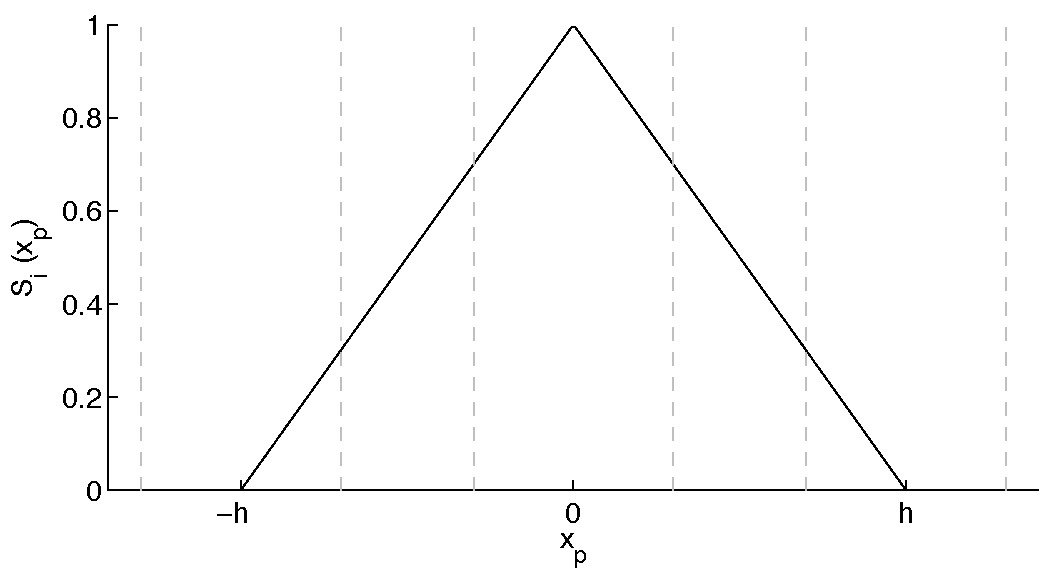
\includegraphics[scale=.85]{mpm_basis.pdf}
  \caption{Effective shape function when using traditional MPM.}
  \label{Fig:MPMShape}
\end{figure}

\begin{figure}
  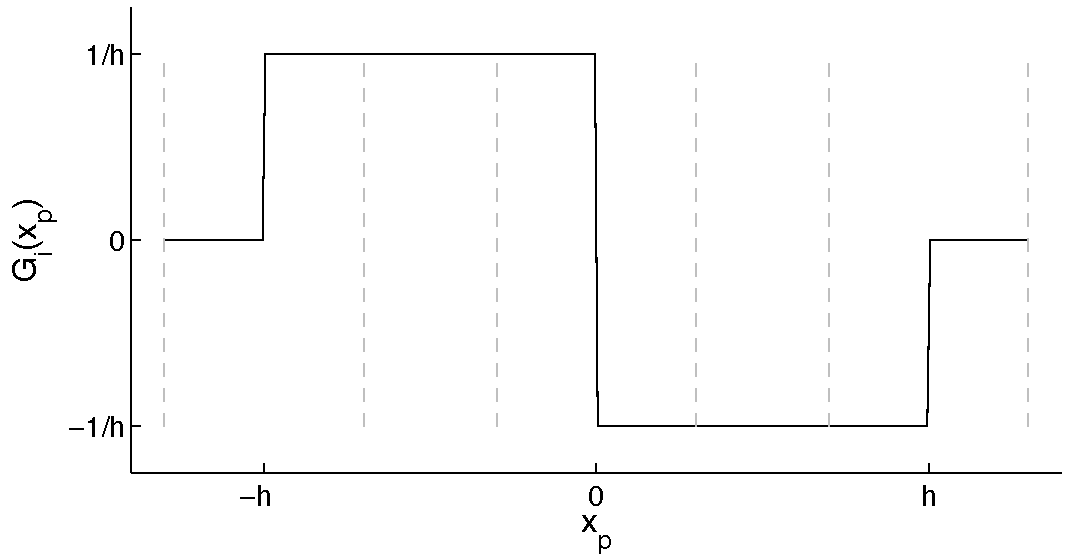
\includegraphics[scale=.85]{mpm_grad.pdf}
  \caption{Gradient of the effective shape function when using traditional MPM.}
  \label{Fig:MPMShapeGrad}
\end{figure}

Typically, when an analyst indicates that
they are ``using GIMP" this implies use of the linear grid basis function
given in Eq.~\ref{linear_shape} and a ``top-hat" characteristic function,
given by (in one-dimension),
\begin{equation}
\chi_p(x) = H(x-(x_p-l_p))-H(x-(x_p+l_p)) , \label{GIMP_char}
\end{equation}
where $H(x)$ is the Heaviside function
($H(x)=0$ if $x<0$ and $H(x)=1$ if $x\ge0$) and $l_p$ is the half-length
of the particle.  When the convolution indicated in Eq.~\ref{effectiveS}
is carried out using the expressions in Eqns.~\ref{linear_shape}
 and~\ref{GIMP_char}, a closed form for the effective shape function can be
written as:
\begin{equation}
S_{i}\left(x_p\right) = \begin{cases}
   \frac{\left(h+l_p+\left(x_p-x_i\right)\right)^2}{4hl_p} & {-h -l_p < x_p-x_i \le -h+l_p} \\
   1 + \frac{\left(x_p-x_i\right)}{h} & {-h + l_p < x_p-x_i \le -l_p} \\
   1 - \frac{\left(x_p-x_i\right)^2 + l_p^2}{2hl_p} & {-l_p < x_p-x_i \le l_p} \\
   1 - \frac{\left(x_p-x_i\right)}{h} & {l_p  < x_p-x_i \le h-l_p} \\
   \frac{\left(h+l_p-\left(x_p-x_i\right)\right)^2}{4hl_p} & {h -l_p < x_p-x_i \le h+l_p} \\
   0 & \text{otherwise},
\end{cases}
\label{gimp_shape}
\end{equation}
%
The gradient of which is:
\begin{equation}
G_i(x_p) = \begin{cases}
   \frac{h+l_p+\left(x_p-x_i\right)}{2 h l_p} & {-h -l_p < x_p-x_i \le -h+l_p} \\
   \frac{1}{h} & {-h + l_p < x_p-x_i \le -l_p} \\
   - \frac{\left(x_p-x_i\right)}{h l_p} & {-l_p < x_p-x_i \le l_p} \\
   - \frac{1}{h} & {l_p  < x_p-x_i \le h-l_p} \\
   - \frac{h+l_p-\left(x_p-x_i\right)}{2 h l_p} & {h -l_p < x_p-x_i \le h+l_p} \\
   0 & \text{otherwise},
\end{cases}
\label{gimpGrad}
\end{equation}

Plots of Equations~\ref{gimp_shape} and~\ref{gimpGrad} are shown
below.  The continuous nature of the gradients are largely responsible
for the improved robustness and accuracy of GIMP over MPM.

\begin{figure}
  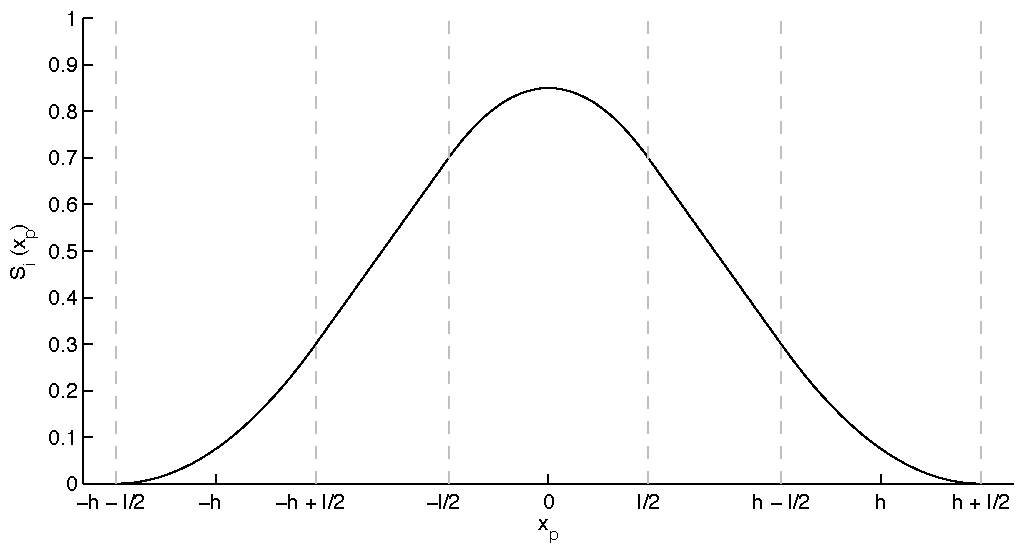
\includegraphics[scale=.85]{gimp_basis.pdf}
  \caption{Effective shape function when using GIMP.}
  \label{Fig:GIMP}
\end{figure}

\begin{figure}
  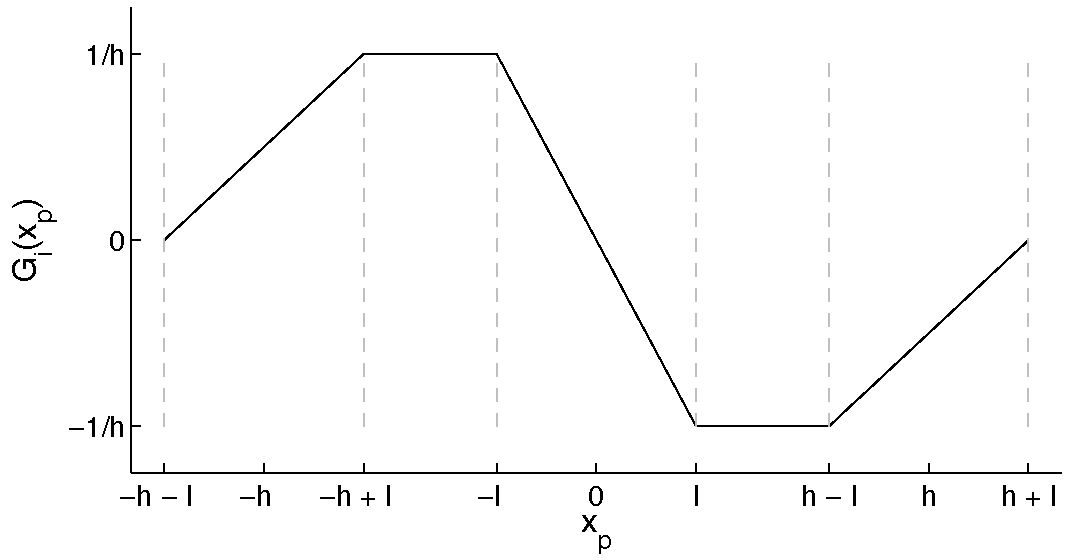
\includegraphics[scale=.85]{gimp_grad.pdf}
  \caption{Gradient of the effective shape function when using GIMP.}
  \label{Fig:GradGIMP}
\end{figure}
%
There is one further consideration in defining the effective shape function,
and that is whether or not the size (length in 1-D) of the particle is kept
fixed (denoted as ``UGIMP" here)
or is allowed to evolve due to material deformations 
(``Finite GIMP" or ``Contiguous GIMP" in (1) and ``cpGIMP" here).
In one-dimensional
simulations, evolution of the particle (half-)length is straightforward,
\begin{equation}
l_p^n = F_p^n l_p^0 ,  \label{particle_length}
\end{equation} 
where $F_p^n$ is the deformation gradient at time $n$.
In multi-dimensional simulations, a similar approach can be used, assuming
an initially rectangular or cuboid particle, to find the current particle
shape.  The difficulty arises in evaluating Eq.~\ref{effectiveS} for
these general shapes.  One approach, apparently effective, has been to create
a cuboid that circumscribes the deformed particle shape~\cite{jinmaCMES2006}.
Alternatively, one can assume that the particle size remains constant (insofar
as it applies to the effective shape function evaluations only).  This is
the approach currently implemented in Uintah.

\subsection{Uintah Implementation} \label{Sec:UintahImp}

Users of Uintah-MPM needn't necessarily bother themselves with the
implementation in code of the algorithm described above.  This section
is intended to serve as a reference for users who find themselves needing
to modify the source code, or those who are simply interested.  Anyone
just wishing to run MPM simulations may skip ahead to
Sections~\ref{Sec:UintahSpecMPM} and~\ref{Sec:ExamplesMPM}.  The goal of
this section is to provide a mapping from the the algorithm described above
to the software that carries it out.  This won't be exhaustive, but will be a
good starting point for the motivated reader.

The source code for the Uintah-MPM implementation can be found in

\begin{Verbatim}[fontsize=\footnotesize]
src/CCA/Components/MPM
\end{Verbatim}

Within that directory are a number of files and subdirectories, these will be
discussed as needed.  For the moment, consider the various files that end in
``{MPM.cc}":
\begin{Verbatim}[fontsize=\footnotesize]
AMRMPM.cc  FractureMPM.cc  ImpMPM.cc  RigidMPM.cc  SerialMPM.cc  ShellMPM.cc
\end{Verbatim}

\tt AMRMPM.cc \normalfont is the nascent beginnings of an AMR implementation of MPM. 
It is far from complete and should be ignored.  \tt FractureMPM.cc \normalfont is an implementation of
the work of Guo and Nairn \cite{GuoNairn}, and while it is viable, it is
undocumented and unsupported.  \tt ShellMPM.cc \normalfont is a treatment of MPM particles
as shell and membrane elements, developed by Biswajit Bannerjee.  It is also
viable, but also undocumented and unsupported.  \tt ImpMPM.cc \normalfont is an implicit
time integration form of MPM based on the work of Guilkey and Weiss
\cite{Guilkey03}.  It is also viable, and future releases of Uintah will include
documentation of its capabilities and uses.  For now, interested readers
should contact Jim Guilkey directly for more information.  \tt RigidMPM.cc \normalfont contains
a very reduced level of functionality, and is used solely in conjunction with
the MPMArches component.

This leaves \tt SerialMPM.cc. \normalfont  This contains, despite its name, the parallel
implementation of the algorithm described above in Section~\ref{Sec:AlgDesc}.
For now, we will skip over the initialization procedures such as:
\begin{Verbatim}[fontsize=\footnotesize]
SerialMPM::problemSetup
SerialMPM::scheduleInitialize
SerialMPM::actuallyInitialize
\end{Verbatim}
and focus mainly on the timestepping algorithm described above.  Reference
will be made back to these functions as needed in
Section~\ref{Sec:UintahSpecMPM}.

Each of the Uintah components contains a function called  \tt scheduleTimeAdvance \normalfont.
The algorithms implemented in these components are broken into a number
of steps.  The implementation of these steps in Uintah take place in ``tasks".
Each task is responsible for performing the calculations needed to accomplish
that step in the algorithm.  Thus, each task requires some data upon which
to operate, and it also creates some data, either as a final result, or as
input to a subsequent task.  Before individual tasks are executed, each is
first ``scheduled".  The scheduling of tasks describes the dataflow and data
dependencies for a given algorithm.  By describing the data dependencies,
both temporally and spatially, each task can be executed in the proper order,
and communication tasks can automatically be generated by the Uintah
infrastructure to achieve parallelism.  Thus, scheduleTimeAdvance calls
a series of functions, each of which schedules the individual tasks.  Let's
begin by looking at the \tt scheduleTimeAdvance \normalfont for \tt SerialMPM, \normalfont pasted below.

\begin{Verbatim}[fontsize=\footnotesize]
void
SerialMPM::scheduleTimeAdvance(const LevelP & level,
                               SchedulerP   & sched)
{
  MALLOC_TRACE_TAG_SCOPE("SerialMPM::scheduleTimeAdvance()");
  if (!flags->doMPMOnLevel(level->getIndex(), level->getGrid()->numLevels()))
    return;

  const PatchSet* patches = level->eachPatch();
  const MaterialSet* matls = d_sharedState->allMPMMaterials();

  scheduleApplyExternalLoads(             sched, patches, matls);
  scheduleInterpolateParticlesToGrid(     sched, patches, matls);
  scheduleExMomInterpolated(              sched, patches, matls);
  scheduleComputeContactArea(             sched, patches, matls);
  scheduleComputeInternalForce(           sched, patches, matls);

  scheduleComputeAndIntegrateAcceleration(sched, patches, matls);
  scheduleExMomIntegrated(                sched, patches, matls);
  scheduleSetGridBoundaryConditions(      sched, patches, matls);
  scheduleSetPrescribedMotion(            sched, patches, matls);
  scheduleComputeStressTensor(            sched, patches, matls);
  if(flags->d_doExplicitHeatConduction){
    scheduleComputeHeatExchange(          sched, patches, matls);
    scheduleComputeInternalHeatRate(      sched, patches, matls);
    scheduleComputeNodalHeatFlux(         sched, patches, matls);
    scheduleSolveHeatEquations(           sched, patches, matls);
    scheduleIntegrateTemperatureRate(     sched, patches, matls);
  }
  scheduleAddNewParticles(                sched, patches, matls);
  scheduleConvertLocalizedParticles(      sched, patches, matls);
  scheduleInterpolateToParticlesAndUpdate(sched, patches, matls);

  if(flags->d_canAddMPMMaterial){
    //  This checks to see if the model on THIS patch says that it's
    //  time to add a new material
    scheduleCheckNeedAddMPMMaterial(         sched, patches, matls);

    //  This one checks to see if the model on ANY patch says that it's
    //  time to add a new material
    scheduleSetNeedAddMaterialFlag(         sched, level,   matls);
  }

  sched->scheduleParticleRelocation(level, lb->pXLabel_preReloc,
                                    d_sharedState->d_particleState_preReloc,
                                    lb->pXLabel,
                                    d_sharedState->d_particleState,
                                    lb->pParticleIDLabel, matls);
  if(d_analysisModule){
    d_analysisModule->scheduleDoAnalysis( sched, level);
  }
}
\end{Verbatim}

The preceding includes scheduling for a number of rarely used features.
For now, let's condense the preceding to the essential tasks:

\begin{Verbatim}[fontsize=\footnotesize]
void
SerialMPM::scheduleTimeAdvance(const LevelP & level,
                               SchedulerP   & sched)
{
  if (!flags->doMPMOnLevel(level->getIndex(), level->getGrid()->numLevels()))
    return;

  const PatchSet* patches = level->eachPatch();
  const MaterialSet* matls = d_sharedState->allMPMMaterials();

  scheduleApplyExternalLoads(             sched, patches, matls);
  scheduleInterpolateParticlesToGrid(     sched, patches, matls);
  scheduleExMomInterpolated(              sched, patches, matls);
  scheduleComputeInternalForce(           sched, patches, matls);

  scheduleComputeAndIntegrateAcceleration(sched, patches, matls);
  scheduleExMomIntegrated(                sched, patches, matls);
  scheduleSetGridBoundaryConditions(      sched, patches, matls);
  scheduleComputeStressTensor(            sched, patches, matls);
  scheduleInterpolateToParticlesAndUpdate(sched, patches, matls);

  sched->scheduleParticleRelocation(level, lb->pXLabel_preReloc,
                                    d_sharedState->d_particleState_preReloc,
                                    lb->pXLabel,
                                    d_sharedState->d_particleState,
                                    lb->pParticleIDLabel, matls);
}
\end{Verbatim}

As described above, each of the ``schedule" functions describes dataflow,
and it also calls the function that actually executes the task.  The naming
convention is illustrated by an example,
\tt scheduleComputeAndIntegrateAcceleration \normalfont calls \tt computeAndIntegrateAcceleration. \normalfont
Let's examine this particular task, which executes
Equations~\ref{MPM:acceleration} and~\ref{MPM:euler}, more carefully.  First,
the scheduling of the task:

\begin{Verbatim}[fontsize=\footnotesize]
void SerialMPM::scheduleComputeAndIntegrateAcceleration(SchedulerP& sched,
                                                       const PatchSet* patches,
                                                       const MaterialSet* matls)
{
  if (!flags->doMPMOnLevel(getLevel(patches)->getIndex(),
                           getLevel(patches)->getGrid()->numLevels()))
    return;

  printSchedule(patches,cout_doing,"MPM::scheduleComputeAndIntegrateAcceleration\t\t\t\t");

  Task* t = scinew Task("MPM::computeAndIntegrateAcceleration",
                        this, &SerialMPM::computeAndIntegrateAcceleration);

  t->requires(Task::OldDW, d_sharedState->get_delt_label() );

  t->requires(Task::NewDW, lb->gMassLabel,          Ghost::None);
  t->requires(Task::NewDW, lb->gInternalForceLabel, Ghost::None);
  t->requires(Task::NewDW, lb->gExternalForceLabel, Ghost::None);
  t->requires(Task::NewDW, lb->gVelocityLabel,      Ghost::None);

  t->computes(lb->gVelocityStarLabel);
  t->computes(lb->gAccelerationLabel);

  sched->addTask(t, patches, matls);
}
\end{Verbatim}

The \tt if \normalfont statement basically directs the schedule to only do this task on the 
finest level (MPM can be used in AMR simulations, but only at the finest
level.)  The \tt printSchedule \normalfont command is in place for debugging purposes,
this type of print statement can be turned on by setting an environmental
variable.  The real business of this task begins with the declaration of the
Task.  In the task declaration, the function associated with that task is
identified.  Subsequent to that is a description of the data dependencies.
Namely, this task \tt requires \normalfont the mass, internal and external forces as well
as velocity on the grid.  No ghost data are required as this task is a 
node by node calculation.  It also requires the timestep size.  Note also
that most of the required data are needed from the \tt NewDW \normalfont where
\tt DW \normalfont refers to
DataWarehouse.  This simply means that these data were calculated by an
earlier task in the current timestep.  The timestep size for this step
was computed in the previous timestep, and thus is required from the \tt OldDW. \normalfont
Finally, this task \tt computes \normalfont the acceleration and time advanced velocity
at each node.

The code to execute this task is as follows:

\begin{Verbatim}[fontsize=\footnotesize]
void SerialMPM::computeAndIntegrateAcceleration(const ProcessorGroup*,
                                                const PatchSubset* patches,
                                                const MaterialSubset*,
                                                DataWarehouse* old_dw,
                                                DataWarehouse* new_dw)
{
  for(int p=0;p<patches->size();p++){
    const Patch* patch = patches->get(p);
    printTask(patches, patch,cout_doing,"Doing computeAndIntegrateAcceleration\t\t\t\t");

    Ghost::GhostType  gnone = Ghost::None;
    Vector gravity = d_sharedState->getGravity();
    for(int m = 0; m < d_sharedState->getNumMPMMatls(); m++){
      MPMMaterial* mpm_matl = d_sharedState->getMPMMaterial( m );
      int dwi = mpm_matl->getDWIndex();

      // Get required variables for this patch
      constNCVariable<Vector> internalforce, externalforce, velocity;
      constNCVariable<double> mass;

      delt_vartype delT;
      old_dw->get(delT, d_sharedState->get_delt_label(), getLevel(patches) );

      new_dw->get(internalforce,lb->gInternalForceLabel, dwi, patch, gnone, 0);
      new_dw->get(externalforce,lb->gExternalForceLabel, dwi, patch, gnone, 0);
      new_dw->get(mass,         lb->gMassLabel,          dwi, patch, gnone, 0);
      new_dw->get(velocity,     lb->gVelocityLabel,      dwi, patch, gnone, 0);

      // Create variables for the results
      NCVariable<Vector> velocity_star,acceleration;
      new_dw->allocateAndPut(velocity_star, lb->gVelocityStarLabel, dwi, patch);
      new_dw->allocateAndPut(acceleration,  lb->gAccelerationLabel, dwi, patch);

      acceleration.initialize(Vector(0.,0.,0.));
      double damp_coef = flags->d_artificialDampCoeff;

      for(NodeIterator iter=patch->getExtraNodeIterator__New();
                        !iter.done();iter++){
        IntVector c = *iter;
        Vector acc(0.,0.,0.);
        if (mass[c] > flags->d_min_mass_for_acceleration){
          acc  = (internalforce[c] + externalforce[c])/mass[c];
          acc -= damp_coef*velocity[c];
        }
        acceleration[c] = acc +  gravity;
        velocity_star[c] = velocity[c] + acceleration[c] * delT;
      }
    }    // matls
  }
}
\end{Verbatim}

This task contains three nested for loops.  First, is a loop over all of the
``patches" that the processor executing this task is responsible for.  Next
is a loop over all materials (imagine a simulation involving the interaction
between, say, tungsten and copper).  Within this loop, the required data
are retrieved from the \tt new\_dw \normalfont (New DataWarehouse) and space for the data
to be created is allocated.  The final loop is over all of the nodes on
the current patch, and the calculations described by
Equations~\ref{MPM:acceleration} and~\ref{MPM:euler} are carried out.  (This
also includes a linear damping term not described above.)

Let's consider each task in turn.  The remaining tasks will be described
in much less detail, but the preceding dissection of a fairly simple task,
along with a description of what the remaining tasks are intended to 
accomplish, should allow interested individuals to follow the remainder
of the Uintah-MPM implementation.

\begin{enumerate}
\item {\tt scheduleApplyExternalLoads \normalfont} This task is mainly responsible for
applying traction boundary conditions described in the input file.  This is
done by assigning external force vectors to the particles.  If the user
wishes to apply a load that is not possible to acheive via the input file
options, it is straightforward to modify the code here to do ``one-off" tests.

\item {\tt scheduleInterpolateParticlesToGrid \normalfont}   The name of this task was
poorly chosen, but has persisted.  This task carries out the operations given
in Equation~\ref{accumulate}.  It also sets boundary conditions on some of
the variables, such as the grid temperature, and grid velocity 
(in the case of symmetry BCs).

\item {\tt scheduleExMomInterpolated \normalfont}  This task actually exists in one
of the contact models which can be found in the \tt Contact \normalfont directory.  Each of those
models has two main tasks. This is the the first of those. It is responsible
for modifying the grid velocity computed by interpolateParticlesToGrid according
to the rules for the particular contact model chosen in the input file.  These
models are briefly described in Section~\ref{Contact}. 

\item {\tt scheduleComputeInternalForce \normalfont} This task computes the volume
integral of the divergence of stress.  Specifically, it carries out the
operation given in Equation~\ref{computeIntForce}.  It also computes some
diagnostic data, if requested in the input file, such as the reaction forces
(tractions) on the boundaries of the computational domain.

\item {\tt scheduleComputeAndIntegrateAcceleration \normalfont} As described previously,
this task carries out the operations described in 
Equations~\ref{MPM:acceleration} and~\ref{MPM:euler}.

\item {\tt scheduleExMomIntegrated \normalfont}  This is the second of the contact tasks
(see above).  It is responsible for modifiying the time advanced grid velocity
computed in \tt computeAndIntegrateAcceleration. \normalfont

\item {\tt scheduleSetGridBoundaryConditions \normalfont}  This task sets boundary conditions
on the time advanced grid velocity.  It also sets an acceleration boundary
condition as well.  However, rather than just setting the acceleration
to a given value, it is computed by solving Equation~\ref{MPM:euler} for
acceleration, and then recomputing the acceleration (on all nodes) as:
\begin{eqnarray}
\bfa_i= \frac{\bfv^L_i - \bfv_i}{\Delta{t}}
\label{MPM:accBC}
\end{eqnarray}
Doing this operation on all nodes has several advantages.  For most interior
nodes, the value for acceleration will be unchanged, but for nodes on the 
where the velocity has been altered by enforcing boundary conditions, and
for nodes at which the contact models have altered the velocity, the acceleration
will be modified to reflect that alteration.

\item{\tt scheduleComputeStressTensor \normalfont}  The task, \tt computeStressTensor, \normalfont
exists in each of the models in the \tt ConstitutiveModel \normalfont directory.  Each
model is responsible for carrying out the operations given in
Equation~\ref{p_vol}, and of course, as the name implies, it also computes
the material stress.  This task has one additional important function,
and that is computing the timestep size for the subsequent step.  The CFL
condition dictates that the timestep size be limited according to:
\begin{eqnarray}
\Delta{t} < \frac{\Delta{x}}{c+|u|}
\label{MPM:CFL}
\end{eqnarray}
where $\Delta{x}$ is the cell spacing, $c$ is the wavespeed in the material,
and $|u|$ is the magnitude of the local velocity.  Because the wavespeed 
may depend on the state of stress that a material is in, this task provides
a convenient time at which to make this calculation.  A timestep size is
computed for all particles, and the minimum for the particle set on a given
patch is put into a ``reduction variable".  The Uintah infrastructure then
does a global reduction to select the smallest timestep from across the
domain.

\item {\tt scheduleInterpolateToParticlesAndUpdate \normalfont}  This task carries out the
operations in Equations~\ref{MPM:updateVp} and~\ref{MPM:updateXp}, namely updating
the particle state based on the grid solution.

\item {\tt scheduleParticleRelocation \normalfont}  This task is not actually located
in the MPM code, but in the Uintah infrastructure.  The idea is that as particles
move, some will cross patch boundaries, and their data will need to be sent to
other processors.  This task is responsible for identifying particles that have
left the patch that they were on, finding where they went, and sending their
data to the correct processor.

\end{enumerate}



\subsection{Uintah Specification} \label{Sec:UintahSpecMPM}

\subsubsection{Basic Inputs}
\subsubsection{Physical Constants}
\subsubsection{Material Properties}
\subsubsection{Constitutive Models} \label{ConstitutiveModels}
\subsubsection{Contact}  \label{Contact}
\subsubsection{BoundaryConditions}
\subsubsection{Physical Boundary Conditions} \label{PhysicalBCs}
\subsubsection{On the Fly Analysis} \label{OTFA_MPM}

\subsection{Examples} \label{Sec:ExamplesMPM}

\subsection{References}
\bibliographystyle{plain}
\bibliography{mpm}







